\documentclass[a4paper,11pt]{amsart}

\usepackage{mathrsfs}
\usepackage{gensymb}
\usepackage{circuitikz}
\usepackage{tikz}
\usetikzlibrary{arrows.meta}
\usepackage{caption}
%\usepackage{newtxmath}
%\usepackage{txfonts}
\usepackage{times}
\usepackage[top=27mm, left=23mm, bottom=23mm, right=23mm]{geometry}
\usepackage{amsfonts, amssymb, amsgen, amsthm, amscd, amsmath}
\usepackage{mathtools}
\mathtoolsset{showonlyrefs=true}
%\usepackage{pxfonts}
\usepackage{bm}
%\usepackage{mathpazo}
\usepackage{domitian}
\usepackage[T1]{fontenc}
\usepackage{upgreek}
\let\oldstylenums\oldstyle

\usepackage{enumerate}
\usepackage{color}
\usepackage[all]{xy}

\newtheorem{theorem}{Theorem}[section]
\newtheorem{proposition}[theorem]{Proposition}
\newtheorem{lemma}[theorem]{Lemma}
\newtheorem{corollary}[theorem]{Corollary}
\newtheorem{claim}[theorem]{Claim}
\theoremstyle{definition}
\newtheorem{remark}[theorem]{Remark}
\newtheorem{example}[theorem]{Example}
\newtheorem{definition}[theorem]{Definition}

\newcommand{\outimes}[2]{\overset{#1}{\underset{#2}{\otimes}}}
\newcommand{\C}[1]{\mathcal{#1}}
\newcommand{\B}[1]{\mathbb{#1}}
\newcommand{\G}[1]{\mathfrak{#1}}
\newcommand{\rmod}[1]{\text{{\bf Mod}-}{#1}}

\newcommand{\Span}{\text{\rm Span}}
\newcommand{\Tor}{\text{\rm Tor}}
\newcommand{\Ind}{\text{\rm Ind}}
\newcommand{\Res}{\text{\rm Res}}
\newcommand{\Ext}{\text{\rm Ext}}
\newcommand{\Hom}{\text{\rm Hom}}
\newcommand{\CoInd}{\text{\rm CoInd}}
\newcommand{\Simp}{{\Delta}}
\newcommand{\Diff}{{\Omega}}
\newcommand{\xla}[1]{\xleftarrow{#1}}
\newcommand{\colim}{\text{colim}}
\renewcommand{\baselinestretch}{1.15}
\renewcommand\parallel{\mathrel{/\mskip-2.5mu/}}
\setlength{\parskip}{1.2mm}
\setlength{\parindent}{0mm}

\title{Electromagnetism Assignment For The Third Time}

\author{Haixuan Lin - 23307110267}
\email{23307110267@m.fudan.edu.cn}


\address{Fudan University, Physics Department, China}

\begin{document}
	
	\begin{abstract}
		Here is the electromagnetism assignment for the third time which is for the corse given by professor Weichao Liu. In order to practise the expertise in scientific film of physics, students need to practise using \LaTeX to composing their own work, even if this is only a ordinary homework.
	\end{abstract}
	
	\maketitle
	
	\section*{Main Text}
		
	\subsection*{2-4}
	\subsubsection*{(1)}
	$C$, $D$ plates are not charged, so the sum of the electric field vectors they generate is $\bm{0}$ and does not change the spatial potential distribution.
	$$
	U_{AC}=U_{CD}=U_{DB}=\frac{1}{3}U_0
	$$
	$$
	E_{AC}=E_{CD}=E_{DB}=\frac{U_0}{d}
	$$
	\subsubsection*{(2)}
	
	The opposite charges between the $CD$ plate are neutralized, but the opposite charges between the $AC$ plate and the DB plate remain unchanged, and the result is that the middle two plates become equivalent to one plate.
	%\begin{figure}[htbp]
		%\begin{minipage}{0.95\textwidth}
			\begin{center}
				
				\tikzset{every picture/.style={line width=0.75pt}} %set default line width to 0.75pt        
				
				\begin{tikzpicture}[x=0.95pt,y=0.95pt,yscale=-1,xscale=1]
					%uncomment if require: \path (0,300); %set diagram left start at 0, and has height of 300
					
					%Shape: Capacitor [id:dp011936745609759658] 
					\draw   (189,159) -- (225,159) (233,139) -- (233,179) (225,139) -- (225,179) (233,159) -- (269,159) ;
					%Shape: Capacitor [id:dp775638037183086] 
					\draw   (145,159) -- (181,159) (189,139) -- (189,179) (181,139) -- (181,179) (189,159) -- (225,159) ;
					%Shape: Capacitor [id:dp018939236807596238] 
					\draw   (318,160) -- (373.8,160) (386.2,140) -- (386.2,180) (373.8,140) -- (373.8,180) (386.2,160) -- (442,160) ;
					%Straight Lines [id:da13921702155965754] 
					\draw    (282,160) -- (306.11,159.78) ;
					\draw [shift={(308.11,159.76)}, rotate = 179.47] [color={rgb, 255:red, 0; green, 0; blue, 0 }  ][line width=0.75]    (10.93,-3.29) .. controls (6.95,-1.4) and (3.31,-0.3) .. (0,0) .. controls (3.31,0.3) and (6.95,1.4) .. (10.93,3.29)   ;				
				\end{tikzpicture}
				
				\captionof*{figure}{Equivalent To One Plate} % 需要 caption 宏包
				
				% 或者如果不想用 caption 宏包:
				%\textbf{BE}
				%	\end{minipage}
				%\end{figure}
				
			\end{center}
			
			
	As a result:
	$$
	U_{AC}=U_{DB}=\frac{1}{3}U_0
	$$
	$$
	E_{AC}=E_{DB}=\frac{U_0}{d}
	$$
	$$
	U_{CD}=0\vphantom{\frac{1}{3}U_0}
	$$
	$$
	E_{CD}=0\vphantom{\frac{U_0}{d}}
	$$
	\subsubsection*{(3)}
	Let the final charge distribution be as shown.
	
	\begin{center}
		
		
		\tikzset{every picture/.style={line width=0.75pt}} %set default line width to 0.75pt        
		
		\begin{tikzpicture}[x=0.75pt,y=0.75pt,yscale=-1,xscale=1]
			%uncomment if require: \path (0,302); %set diagram left start at 0, and has height of 302
			
			%Straight Lines [id:da8443995923714569] 
			\draw    (220.44,61.33) -- (220.44,218.18) ;
			%Straight Lines [id:da1696805536031114] 
			\draw    (312.36,62.76) -- (310.95,221.03) ;
			%Straight Lines [id:da9421444265926342] 
			\draw    (407.11,65.14) -- (407.11,218.18) ;
			%Straight Lines [id:da5789108810821422] 
			\draw    (500.44,62.28) -- (500.44,215.32) ;
			%Curve Lines [id:da00023792255473420454] 
			\draw    (278.56,222) .. controls (318.16,192.3) and (268.02,220.15) .. (305.83,191.6) ;
			\draw [shift={(307,190.72)}, rotate = 143.13] [color={rgb, 255:red, 0; green, 0; blue, 0 }  ][line width=0.75]    (10.93,-3.29) .. controls (6.95,-1.4) and (3.31,-0.3) .. (0,0) .. controls (3.31,0.3) and (6.95,1.4) .. (10.93,3.29)   ;
			%Curve Lines [id:da22681088082087708] 
			\draw    (441,221.72) .. controls (412.87,186.97) and (448.89,211.95) .. (421.3,183.08) ;
			\draw [shift={(420,181.72)}, rotate = 45.94] [color={rgb, 255:red, 0; green, 0; blue, 0 }  ][line width=0.75]    (10.93,-3.29) .. controls (6.95,-1.4) and (3.31,-0.3) .. (0,0) .. controls (3.31,0.3) and (6.95,1.4) .. (10.93,3.29)   ;
			%Curve Lines [id:da13833471471663672] 
			\draw    (337,63.72) .. controls (300.37,91.44) and (359.79,63.3) .. (322.17,95.72) ;
			\draw [shift={(321,96.72)}, rotate = 319.64] [color={rgb, 255:red, 0; green, 0; blue, 0 }  ][line width=0.75]    (10.93,-3.29) .. controls (6.95,-1.4) and (3.31,-0.3) .. (0,0) .. controls (3.31,0.3) and (6.95,1.4) .. (10.93,3.29)   ;
			%Curve Lines [id:da9285029024301967] 
			\draw    (388,65.72) .. controls (379.5,73.28) and (392.42,76.38) .. (400.62,83.45) ;
			\draw [shift={(402,84.72)}, rotate = 225] [color={rgb, 255:red, 0; green, 0; blue, 0 }  ][line width=0.75]    (10.93,-3.29) .. controls (6.95,-1.4) and (3.31,-0.3) .. (0,0) .. controls (3.31,0.3) and (6.95,1.4) .. (10.93,3.29)   ;
			
			% Text Node
			\draw (196,42.94) node [anchor=north west][inner sep=0.75pt]   [align=left] {$\displaystyle Q-\Delta Q$};
			% Text Node
			\draw (245,224.94) node [anchor=north west][inner sep=0.75pt]   [align=left] {$\displaystyle -( Q-\Delta Q$)};
			% Text Node
			\draw (464,43.94) node [anchor=north west][inner sep=0.75pt]   [align=left] {$\displaystyle -( Q-\Delta Q$)};
			% Text Node
			\draw (422,220.94) node [anchor=north west][inner sep=0.75pt]   [align=left] {$\displaystyle Q-\Delta Q$};
			% Text Node
			\draw (249.56,124) node [anchor=north west][inner sep=0.75pt]   [align=left] {};
			% Text Node
			\draw (321.56,45) node [anchor=north west][inner sep=0.75pt]   [align=left] {$\displaystyle -\Delta Q$};
			% Text Node
			\draw (370.56,44) node [anchor=north west][inner sep=0.75pt]   [align=left] {$\displaystyle \Delta Q$};
			
			
		\end{tikzpicture}
		
	\end{center}
	 	Charge $Q$ satisfies the relation:
	 	$$
	 	Qd\propto U_0
	 	$$
	 	What's more, plates $A$ and $B$ have the same potential.
	 	$$
	 	\left( Q-\Delta Q \right) \frac{d}{3}-\Delta Q\frac{d}{3}+\left( Q-\Delta Q \right) \frac{d}{3}=0
	 	$$
	 	So $\Delta Q=\dfrac{2}{3}Q.$ And as result:
	 	$$
	 	U_{AC}=U_{DB}=\frac{1}{9}U_0
	 	$$
	 	$$
	 	E_{AC}=E_{DB}=\frac{1}{3}\frac{U_0}{d}
	 	$$
	 	$$
	 	U_{CD}=-\frac{2}{9}U_0
	 	$$
	 	$$
	 	E_{CD}=-\frac{2}{3}\frac{U_0}{d}
	 	$$
	\subsubsection*{(4)}
	The answer of (1) is not change. The answer of (2) will change to
	$$
	U_{AC}=U_{DB}=\frac{1}{2}U_0
	$$
	$$
	E_{AC}=E_{DB}=\frac{3}{2}\frac{U_0}{d}
	$$
	$$
	U_{CD}=0\vphantom{\frac{1}{3}U_0}
	$$
	$$
	E_{CD}=0\vphantom{\frac{U_0}{d}}
	$$
	So as to remain maintain the voltage between $A$ and $B$ is still $U_0$. And the answer of (3) will change to
	$$
	U_{AC}=U_{DB}=\frac{1}{6}U_0
	$$
	$$
	E_{AC}=E_{DB}=\frac{1}{2}\frac{U_0}{d}
	$$
	$$
	U_{CD}=-\frac{1}{3}U_0
	$$
	$$
	E_{CD}=-\frac{U_0}{d}
	$$
	Because it just like the initial charge changes to 1.5 times.
	\subsection*{2-5}
	In order for there to be no charge inside the conductor, the field lines generated by $-q$ must all converge to the induced charge inside the shell, so the induced charge inside the shell is $q$.
	\begin{center}
		
		
		\tikzset{every picture/.style={line width=0.75pt}} %set default line width to 0.75pt        
		
		\begin{tikzpicture}[x=0.75pt,y=0.75pt,yscale=-1,xscale=1]
			%uncomment if require: \path (0,302); %set diagram left start at 0, and has height of 302
			
			%Flowchart: Connector [id:dp6305019052115879] 
			\draw   (263.03,233.82) .. controls (236.53,185.37) and (254.34,124.6) .. (302.79,98.11) .. controls (351.25,71.61) and (412.01,89.41) .. (438.51,137.87) .. controls (465.01,186.33) and (447.2,247.09) .. (398.75,273.59) .. controls (350.29,300.08) and (289.53,282.28) .. (263.03,233.82) -- cycle ;
			%Shape: Circle [id:dp5880513646254804] 
			\draw   (275.77,185.85) .. controls (275.77,144.42) and (309.35,110.85) .. (350.77,110.85) .. controls (392.19,110.85) and (425.77,144.42) .. (425.77,185.85) .. controls (425.77,227.27) and (392.19,260.85) .. (350.77,260.85) .. controls (309.35,260.85) and (275.77,227.27) .. (275.77,185.85) -- cycle ;
			%Straight Lines [id:da6136657541340393] 
			\draw    (350.77,185.85) -- (392,174.72) ;
			
			% Text Node
			\draw (392,160.72) node [anchor=north west][inner sep=0.75pt]   [align=left] {$\displaystyle q$};
			% Text Node
			\draw (397.56,196) node [anchor=north west][inner sep=0.75pt]   [align=left] {$\displaystyle -q$};
			% Text Node
			\draw (459.56,160) node [anchor=north west][inner sep=0.75pt]   [align=left] {$\displaystyle Q+q$};
	
		\end{tikzpicture}		
	\end{center}
	In order for there to be no charge inside the conductor, the field lines generated by -q must all converge to the induced charge inside the shell, so that the distance from each tiny point charge on the shell to the center of the sphere is equal to the local radius, so:
	$$
	U_O=\frac{1}{4\pi \varepsilon _0}\left( \frac{q}{r}-\frac{q}{a}+\frac{Q+q}{b} \right) 
	$$
	\subsection*{2-10}
	\subsubsection*{(1)}
	Just like above.
	\begin{center}
		
		
		\tikzset{every picture/.style={line width=0.75pt}} %set default line width to 0.75pt        
		
		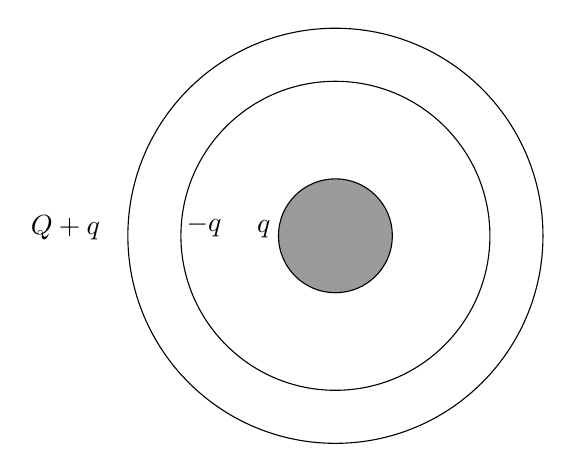
\begin{tikzpicture}[x=0.75pt,y=0.75pt,yscale=-1,xscale=1]
			%uncomment if require: \path (0,302); %set diagram left start at 0, and has height of 302
			
			%Shape: Donut [id:dp02813901889416992] 
			\draw   (105.56,153) .. controls (105.56,111.89) and (138.89,78.56) .. (180,78.56) .. controls (221.11,78.56) and (254.44,111.89) .. (254.44,153) .. controls (254.44,194.11) and (221.11,227.44) .. (180,227.44) .. controls (138.89,227.44) and (105.56,194.11) .. (105.56,153)(80,153) .. controls (80,97.77) and (124.77,53) .. (180,53) .. controls (235.23,53) and (280,97.77) .. (280,153) .. controls (280,208.23) and (235.23,253) .. (180,253) .. controls (124.77,253) and (80,208.23) .. (80,153) ;
			%Shape: Circle [id:dp305941859822344] 
			\draw  [fill={rgb, 255:red, 155; green, 155; blue, 155 }  ,fill opacity=1 ] (152.56,153) .. controls (152.56,137.84) and (164.84,125.56) .. (180,125.56) .. controls (195.16,125.56) and (207.44,137.84) .. (207.44,153) .. controls (207.44,168.16) and (195.16,180.44) .. (180,180.44) .. controls (164.84,180.44) and (152.56,168.16) .. (152.56,153) -- cycle ;
			
			% Text Node
			\draw (141,144.5) node [anchor=north west][inner sep=0.75pt]   [align=left] {$\displaystyle q$};
			% Text Node
			\draw (107,142) node [anchor=north west][inner sep=0.75pt]   [align=left] {$\displaystyle -q$};
			% Text Node
			\draw (32,142) node [anchor=north west][inner sep=0.75pt]   [align=left] {$\displaystyle Q+q$};
			
			
		\end{tikzpicture}
		
	\end{center}
	So:
	$$
	\varphi _2=\frac{1}{4\pi \varepsilon _0}\frac{Q+q}{R_3}
	$$
	And there is no electronic field between $R_3$ and $R_2$ so:
	$$
	\varphi _1=\varphi _2+\frac{1}{4\pi \varepsilon _0}q\left( \frac{1}{R_1}-\frac{1}{R_2} \right) =\frac{1}{4\pi \varepsilon _0}\left( \frac{q}{R_1}-\frac{q}{R_2}+\frac{Q+q}{R_3} \right) 
	$$
	\subsubsection*{(2)}
	$$
	\Delta \varphi=\frac{1}{4\pi \varepsilon _0}\left( \frac{q}{R_1}-\frac{q}{R_2}\right) 
	$$
	\subsubsection*{(3)}
	The $-q$ and $q$ will be combined together as 0, and $\displaystyle\varphi_1=\varphi_2=\frac{1}{4\pi \varepsilon _0}\frac{Q+q}{R_3}$ and $\Delta \varphi =0$.
	
	\subsubsection*{(4)}
	The $Q+q$ will go into the ground and disappear. So $\varphi_2=0$ and $\varphi_1=\displaystyle\frac{q}{4\pi \varepsilon _0}\left( \frac{1}{R_1}-\frac{1}{R_2} \right)$. As a result $\displaystyle\Delta \varphi= \frac{q}{4\pi \varepsilon _0}\left( \frac{1}{R_1}-\frac{1}{R_2} \right) .$
	\subsubsection*{(5)}
	The inter ball and the ground become equipotential bodies so $\varphi_1=0$. Consider the inter ball draw $\Delta q$ from the ground and because the outer ball is far away from ground so 
	$$
	\varphi_2=\frac{1}{4\pi \varepsilon _0}\frac{Q+\Delta q}{R_3}
	$$
	What's more, accoring to electronic field we can get
	$$
	\Delta \varphi =\frac{q+\Delta q}{4\pi \varepsilon _0}\left( \frac{1}{R_1}-\frac{1}{R_2} \right) 
	$$
	And $\varphi _1=\varphi _2+\Delta\varphi=0$. So 
	$$
	\Delta q=\frac{\left( -R_1R_2+R_2R_3-R_3R_1 \right) q-R_1R_2Q}{R_1R_2-R_2R_3+R_3R_1}
	$$
	Take back so we get
	$$
	\varphi _2=-\Delta \varphi =\frac{R_2-R_1}{R_2R_3-R_1R_3+R_1R_2}\frac{Q}{4\pi \varepsilon _0}
	$$
	\subsection*{2-12}
	\subsubsection*{(1)}
	It equals to make the to plate become closer so
	$$
	C=\varepsilon_0\dfrac{S}{d-t}
	$$
	\subsubsection*{(2)}
	Ignoring the boundary effect, it can be seen that there is no effect according to the above equation.
	
	\subsection*{2-14}
	\subsubsection*{(1)}We can think that this is similar to the parallel operation of capacitors.
	$$
	C=C_1\parallel C_2=4\pi \varepsilon_0(a+b)
	$$
	
	\begin{center}
		
		
		\tikzset{every picture/.style={line width=0.75pt}} %set default line width to 0.75pt        
		
		\begin{tikzpicture}[x=0.5pt,y=0.5pt,yscale=-1,xscale=1]
			%uncomment if require: \path (0,300); %set diagram left start at 0, and has height of 300
			
			%Shape: Circle [id:dp5601723616689367] 
			\draw   (19,166) .. controls (19,152.19) and (30.19,141) .. (44,141) .. controls (57.81,141) and (69,152.19) .. (69,166) .. controls (69,179.81) and (57.81,191) .. (44,191) .. controls (30.19,191) and (19,179.81) .. (19,166) -- cycle ;
			%Shape: Circle [id:dp8778461985269816] 
			\draw   (223.67,172.5) .. controls (223.67,158.69) and (234.86,147.5) .. (248.67,147.5) .. controls (262.47,147.5) and (273.67,158.69) .. (273.67,172.5) .. controls (273.67,186.31) and (262.47,197.5) .. (248.67,197.5) .. controls (234.86,197.5) and (223.67,186.31) .. (223.67,172.5) -- cycle ;
			%Shape: Arc [id:dp19034390298149084] 
			\draw  [draw opacity=0] (40.85,78.39) .. controls (40.07,77.3) and (39.67,76.18) .. (39.67,75.04) .. controls (39.67,62.87) and (85.89,53) .. (142.92,53) .. controls (199.94,53) and (246.17,62.87) .. (246.17,75.04) .. controls (246.17,76.78) and (245.22,78.47) .. (243.44,80.1) -- (142.92,75.04) -- cycle ; \draw   (40.85,78.39) .. controls (40.07,77.3) and (39.67,76.18) .. (39.67,75.04) .. controls (39.67,62.87) and (85.89,53) .. (142.92,53) .. controls (199.94,53) and (246.17,62.87) .. (246.17,75.04) .. controls (246.17,76.78) and (245.22,78.47) .. (243.44,80.1) ;  
			%Shape: Arc [id:dp0818054157814565] 
			\draw  [draw opacity=0] (245.34,258.37) .. controls (246.13,259.46) and (246.53,260.58) .. (246.53,261.72) .. controls (246.55,273.89) and (200.34,283.83) .. (143.32,283.92) .. controls (86.3,284.01) and (40.05,274.21) .. (40.03,262.04) .. controls (40.03,260.3) and (40.97,258.61) .. (42.76,256.98) -- (143.28,261.88) -- cycle ; \draw   (245.34,258.37) .. controls (246.13,259.46) and (246.53,260.58) .. (246.53,261.72) .. controls (246.55,273.89) and (200.34,283.83) .. (143.32,283.92) .. controls (86.3,284.01) and (40.05,274.21) .. (40.03,262.04) .. controls (40.03,260.3) and (40.97,258.61) .. (42.76,256.98) ;  
			%Straight Lines [id:da3022933640991108] 
			\draw    (320,170) -- (377,170.08) ;
			\draw [shift={(379,170.08)}, rotate = 180.08] [color={rgb, 255:red, 0; green, 0; blue, 0 }  ][line width=0.75]    (10.93,-3.29) .. controls (6.95,-1.4) and (3.31,-0.3) .. (0,0) .. controls (3.31,0.3) and (6.95,1.4) .. (10.93,3.29)   ;
			%Straight Lines [id:da7448582770300909] 
			\draw    (500,50) -- (500,100) ;
			%Straight Lines [id:da2555410931843065] 
			\draw    (430,100) -- (500,100) ;
			%Straight Lines [id:da4845304235935046] 
			\draw    (500,100) -- (570,100) ;
			%Shape: Capacitor [id:dp5622307923333822] 
			\draw   (430,100) -- (429.99,167.49) (449.99,182.5) -- (409.98,182.49) (449.99,167.5) -- (409.99,167.49) (429.99,182.49) -- (429.97,249.99) ;
			%Shape: Capacitor [id:dp20161418247811858] 
			\draw   (570,100) -- (569.99,167.49) (589.99,182.5) -- (549.98,182.49) (589.99,167.5) -- (549.99,167.49) (569.99,182.49) -- (569.97,249.99) ;
			%Straight Lines [id:da600253192820859] 
			\draw    (499.62,300) -- (500,250) ;
			%Straight Lines [id:da3778928694301904] 
			\draw    (570,250.54) -- (500,250) ;
			%Straight Lines [id:da1898772462956244] 
			\draw    (500,250) -- (430,249.46) ;
			
			% Text Node
			\draw (108.17,30) node [anchor=north west][inner sep=0.75pt]   [align=left] {infinite far};
			
			
		\end{tikzpicture}
		
	\end{center}
	\subsubsection*{(2)}
	The amount of charge on a capacitor is proportional to its size.
	$$
	q_1=\dfrac{a}{a+b}Q
	$$
	$$
	q_2=\dfrac{b}{a+b}Q
	$$
	
	\subsection*{2-19}
	\subsubsection*{(1)}
	Let's consider $\varphi_A=0$ and $\varphi_B=U$. So $Q_4=0$, $Q_1=C_1U$, $Q_2+Q_3=\left( C_2\parallel C_3\right) U$
	$$
	C_{AB}=\dfrac{Q_1+Q_2+Q_3+Q_4}{U}=\frac{C_1C_2+C_2C_3+C_3C_1}{C_2+C_3}
	$$
	\subsubsection*{(2)}
	Just same as above.
	$$
	C_{DE}=\frac{C_1C_2+C_2C_3+C_3C_1}{C_2+C_3}
	$$
	\subsubsection*{(3)}
	Obiously it gets short!
	$$
	C_{AE}=+\infty
	$$
	\subsection*{2-23}
	\subsubsection*{(1)}
	For the $A$ sphere, this corresponds to $A$ scalar superposition of potential.
	$$
	\Delta \varphi_1=\varphi_2
	$$
	For $B$, its outer surface plus $q_1$ so
	$$
	\Delta\varphi_2=\frac{1}{4\pi \varepsilon _0}\frac{q_1}{R_2}=\frac{q_1}{q_2}\varphi _2
	$$
	\subsubsection*{(2)}
	$$
	W=q_1\Delta\varphi_1=q_1\varphi_2
	$$
	\subsection*{3-1}
	Microscopic determination of current:
	$$
	I=neSv
	$$
	So $\displaystyle n=\dfrac{I}{eSv}=1.3\times 10^5\thinspace\mathrm{mm^{-3}}$.
	\subsection*{3-7}
	\subsubsection*{(1)}
	Consider a very thin ball surface.
	$$
	\mathrm{d}R=\rho \frac{\mathrm{d}r}{4\pi r^2}\Longrightarrow R=\int_{r_a}^{r_b}{\mathrm{d}R=\frac{\rho}{4\pi}\left( \frac{1}{r_a}-\frac{1}{r_b} \right)}
	$$
	\subsubsection*{(2)}
	$$
	J(r)=\dfrac{I}{S(r)}=\dfrac{U}{RS(r)}=\frac{r_ar_bU}{\rho \left( r_b-r_a \right) r_2}
	$$
	\subsection*{3-10}
	Examine the definition of resistance.
	$$
	R_{AB}=\dfrac{d_1}{\gamma_1S}\qquad R_{BC}=\dfrac{d_2}{\gamma_2S}
	$$
	Ignoring the marginal effect, the electric field generated by the surface density of charge can be used to find the potential difference.
	$$
	U_{AB}=E_{AB}d_1=\frac{\sigma _A-\sigma _B-\sigma _C}{2\varepsilon _0}d_1\qquad U_{BC}=E_{BC}d_1=\frac{\sigma _A+\sigma _B-\sigma _C}{2\varepsilon _0}d_2
	$$
	Ohm's law:
	$$
	U_{AB}=IR_{AB}\qquad U_{BC}=IR_{BC}
	$$
	And no net charge accumulates on electronic components.
	$$
	\sigma_A+\sigma_B+\sigma_C=0
	$$
	So:
	$$
	\sigma _A=\frac{\varepsilon _0l}{\gamma _1S}\qquad \sigma _B=\frac{\varepsilon _0l}{S}\left( \frac{1}{\gamma _2}-\frac{1}{\gamma _1} \right) \qquad \sigma _C=-\frac{\varepsilon _0l}{\gamma _2S}
	$$
	\subsection*{3-16}
	\subsubsection*{(1)}
	By the definition of current.
	$$
	N=\dfrac{I\Delta t}{e}=3.12\times10^{11}
	$$
	\subsubsection*{(2)}
	$$
	\bar{I}=I\times\dfrac{500\times0.1\times10^{-6}}{1}=25\thinspace\mathrm{\upmu A}
	$$
	\subsubsection*{(3)}
	$$
	\bar{P}=\dfrac{IW_i}{e}=1250\thinspace\mathrm{W}
	$$
	\subsection*{3-20}
	\begin{center}
		
		
		\tikzset{every picture/.style={line width=0.75pt}} %set default line width to 0.75pt        
		
		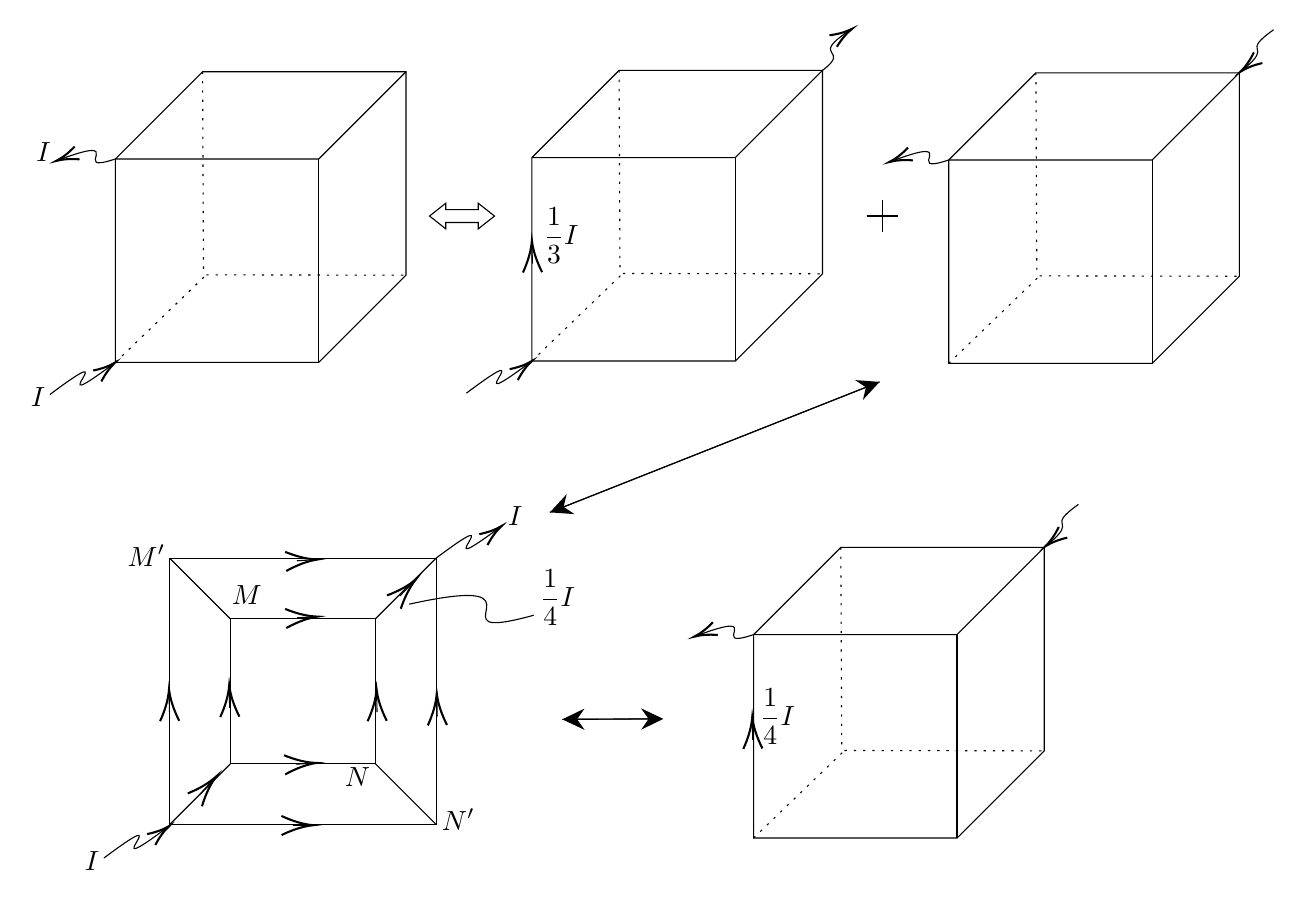
\begin{tikzpicture}[x=0.75pt,y=0.75pt,yscale=-1,xscale=1]
			%uncomment if require: \path (0,777); %set diagram left start at 0, and has height of 777
			
			%Shape: Cube [id:dp5143443825294411] 
			\draw   (98.67,103.33) -- (140.67,61.33) -- (238.67,61.33) -- (238.67,159.33) -- (196.67,201.33) -- (98.67,201.33) -- cycle ; \draw   (238.67,61.33) -- (196.67,103.33) -- (98.67,103.33) ; \draw   (196.67,103.33) -- (196.67,201.33) ;
			%Straight Lines [id:da6286629946044935] 
			\draw  [dash pattern={on 0.84pt off 2.51pt}]  (140.67,61.33) -- (141.11,157.83) ;
			%Straight Lines [id:da5900349206255819] 
			\draw  [dash pattern={on 0.84pt off 2.51pt}]  (142.44,159.17) -- (238.67,159.33) ;
			%Straight Lines [id:da3149705021847309] 
			\draw  [dash pattern={on 0.84pt off 2.51pt}]  (98.67,201.33) -- (142.44,159.17) ;
			%Curve Lines [id:da05630178945288766] 
			\draw    (67.11,216.83) .. controls (106.71,187.13) and (59.63,230.45) .. (97.49,202.21) ;
			\draw [shift={(98.67,201.33)}, rotate = 143.13] [color={rgb, 255:red, 0; green, 0; blue, 0 }  ][line width=0.75]    (10.93,-3.29) .. controls (6.95,-1.4) and (3.31,-0.3) .. (0,0) .. controls (3.31,0.3) and (6.95,1.4) .. (10.93,3.29)   ;
			%Curve Lines [id:da9261428236291769] 
			\draw    (98.67,103.33) .. controls (75.03,111.21) and (106.69,90.63) .. (71.65,103.71) ;
			\draw [shift={(70,104.33)}, rotate = 339.17] [color={rgb, 255:red, 0; green, 0; blue, 0 }  ][line width=0.75]    (10.93,-3.29) .. controls (6.95,-1.4) and (3.31,-0.3) .. (0,0) .. controls (3.31,0.3) and (6.95,1.4) .. (10.93,3.29)   ;
			%Shape: Cube [id:dp6352103238220146] 
			\draw   (299.33,102.67) -- (341.33,60.67) -- (439.33,60.67) -- (439.33,158.67) -- (397.33,200.67) -- (299.33,200.67) -- cycle ; \draw   (439.33,60.67) -- (397.33,102.67) -- (299.33,102.67) ; \draw   (397.33,102.67) -- (397.33,200.67) ;
			%Straight Lines [id:da04708458614780664] 
			\draw  [dash pattern={on 0.84pt off 2.51pt}]  (341.33,60.67) -- (341.78,157.17) ;
			%Straight Lines [id:da7844329356454909] 
			\draw  [dash pattern={on 0.84pt off 2.51pt}]  (343.11,158.5) -- (439.33,158.67) ;
			%Straight Lines [id:da13387988814921736] 
			\draw  [dash pattern={on 0.84pt off 2.51pt}]  (299.33,200.67) -- (343.11,158.5) ;
			%Curve Lines [id:da5329791767950134] 
			\draw    (267.78,216.17) .. controls (307.38,186.47) and (260.29,229.78) .. (298.16,201.54) ;
			\draw [shift={(299.33,200.67)}, rotate = 143.13] [color={rgb, 255:red, 0; green, 0; blue, 0 }  ][line width=0.75]    (10.93,-3.29) .. controls (6.95,-1.4) and (3.31,-0.3) .. (0,0) .. controls (3.31,0.3) and (6.95,1.4) .. (10.93,3.29)   ;
			%Curve Lines [id:da2603137384123775] 
			\draw    (439.33,60.67) .. controls (453.8,49.7) and (432.29,54.81) .. (452.06,41.63) ;
			\draw [shift={(453.67,40.58)}, rotate = 147.2] [color={rgb, 255:red, 0; green, 0; blue, 0 }  ][line width=0.75]    (10.93,-3.29) .. controls (6.95,-1.4) and (3.31,-0.3) .. (0,0) .. controls (3.31,0.3) and (6.95,1.4) .. (10.93,3.29)   ;
			%Shape: Cube [id:dp05202801344565877] 
			\draw   (500.17,103.83) -- (542.17,61.83) -- (640.17,61.83) -- (640.17,159.83) -- (598.17,201.83) -- (500.17,201.83) -- cycle ; \draw   (640.17,61.83) -- (598.17,103.83) -- (500.17,103.83) ; \draw   (598.17,103.83) -- (598.17,201.83) ;
			%Straight Lines [id:da5137510009617317] 
			\draw  [dash pattern={on 0.84pt off 2.51pt}]  (542.17,61.83) -- (542.61,158.33) ;
			%Straight Lines [id:da9996902277915685] 
			\draw  [dash pattern={on 0.84pt off 2.51pt}]  (543.94,159.67) -- (640.17,159.83) ;
			%Straight Lines [id:da6907785892117242] 
			\draw  [dash pattern={on 0.84pt off 2.51pt}]  (500.17,201.83) -- (543.94,159.67) ;
			%Curve Lines [id:da1881933803965139] 
			\draw    (656.67,41.08) .. controls (639.69,53.21) and (657.53,47.46) .. (642.19,60.11) ;
			\draw [shift={(640.67,61.33)}, rotate = 321.63] [color={rgb, 255:red, 0; green, 0; blue, 0 }  ][line width=0.75]    (10.93,-3.29) .. controls (6.95,-1.4) and (3.31,-0.3) .. (0,0) .. controls (3.31,0.3) and (6.95,1.4) .. (10.93,3.29)   ;
			%Curve Lines [id:da6967163321822727] 
			\draw    (500.17,103.83) .. controls (476.53,111.71) and (508.19,91.13) .. (473.15,104.21) ;
			\draw [shift={(471.5,104.83)}, rotate = 339.17] [color={rgb, 255:red, 0; green, 0; blue, 0 }  ][line width=0.75]    (10.93,-3.29) .. controls (6.95,-1.4) and (3.31,-0.3) .. (0,0) .. controls (3.31,0.3) and (6.95,1.4) .. (10.93,3.29)   ;
			%Left Right Arrow [id:dp3731953589729311] 
			\draw   (250,130.83) -- (257.83,124.67) -- (257.83,127.75) -- (273.5,127.75) -- (273.5,124.67) -- (281.33,130.83) -- (273.5,137) -- (273.5,133.92) -- (257.83,133.92) -- (257.83,137) -- cycle ;
			\draw   (460.67,130.83) -- (475.67,130.83)(468.17,123.33) -- (468.17,138.33) ;
			%Straight Lines [id:da7677113617830491] 
			\draw    (299.56,153.72) -- (299.37,144.67) ;
			\draw [shift={(299.33,142.67)}, rotate = 88.85] [color={rgb, 255:red, 0; green, 0; blue, 0 }  ][line width=0.75]    (15.3,-4.61) .. controls (9.73,-1.96) and (4.63,-0.42) .. (0,0) .. controls (4.63,0.42) and (9.73,1.96) .. (15.3,4.61)   ;
			%Shape: Cube [id:dp659720408746088] 
			\draw   (406.17,332.5) -- (448.17,290.5) -- (546.17,290.5) -- (546.17,388.5) -- (504.17,430.5) -- (406.17,430.5) -- cycle ; \draw   (546.17,290.5) -- (504.17,332.5) -- (406.17,332.5) ; \draw   (504.17,332.5) -- (504.17,430.5) ;
			%Straight Lines [id:da7052482754935823] 
			\draw  [dash pattern={on 0.84pt off 2.51pt}]  (448.17,290.5) -- (448.61,387) ;
			%Straight Lines [id:da2951174191632038] 
			\draw  [dash pattern={on 0.84pt off 2.51pt}]  (449.94,388.33) -- (546.17,388.5) ;
			%Straight Lines [id:da2953104621828895] 
			\draw  [dash pattern={on 0.84pt off 2.51pt}]  (406.17,430.5) -- (449.94,388.33) ;
			%Curve Lines [id:da8410620500116042] 
			\draw    (562.67,269.75) .. controls (545.69,281.88) and (563.53,276.12) .. (548.19,288.77) ;
			\draw [shift={(546.67,290)}, rotate = 321.63] [color={rgb, 255:red, 0; green, 0; blue, 0 }  ][line width=0.75]    (10.93,-3.29) .. controls (6.95,-1.4) and (3.31,-0.3) .. (0,0) .. controls (3.31,0.3) and (6.95,1.4) .. (10.93,3.29)   ;
			%Curve Lines [id:da81121424748075] 
			\draw    (406.17,332.5) .. controls (382.53,340.38) and (414.19,319.8) .. (379.15,332.88) ;
			\draw [shift={(377.5,333.5)}, rotate = 339.17] [color={rgb, 255:red, 0; green, 0; blue, 0 }  ][line width=0.75]    (10.93,-3.29) .. controls (6.95,-1.4) and (3.31,-0.3) .. (0,0) .. controls (3.31,0.3) and (6.95,1.4) .. (10.93,3.29)   ;
			%Straight Lines [id:da11507963541564026] 
			\draw    (314,373.33) -- (359.67,373.12) ;
			\draw [shift={(362.67,373.11)}, rotate = 179.74] [fill={rgb, 255:red, 0; green, 0; blue, 0 }  ][line width=0.08]  [draw opacity=0] (10.72,-5.15) -- (0,0) -- (10.72,5.15) -- (7.12,0) -- cycle    ;
			%Straight Lines [id:da9002441694305012] 
			\draw    (357.2,373.07) -- (317,373.31) ;
			\draw [shift={(314,373.33)}, rotate = 359.65] [fill={rgb, 255:red, 0; green, 0; blue, 0 }  ][line width=0.08]  [draw opacity=0] (10.72,-5.15) -- (0,0) -- (10.72,5.15) -- (7.12,0) -- cycle    ;
			%Shape: Square [id:dp41450605180861166] 
			\draw   (124.83,295.67) -- (253.17,295.67) -- (253.17,424) -- (124.83,424) -- cycle ;
			%Shape: Square [id:dp1907922033745728] 
			\draw   (154.04,324.88) -- (223.96,324.88) -- (223.96,394.79) -- (154.04,394.79) -- cycle ;
			%Straight Lines [id:da4824317318084743] 
			\draw    (124.83,295.67) -- (154.04,324.88) ;
			%Straight Lines [id:da4453323708879] 
			\draw    (253.17,295.67) -- (223.96,324.88) ;
			%Straight Lines [id:da7814660987757811] 
			\draw    (154.04,394.79) -- (124.83,424) ;
			%Straight Lines [id:da4662249710151751] 
			\draw    (223.96,394.79) -- (253.17,424) ;
			%Straight Lines [id:da12518179214967073] 
			\draw    (124.72,369.89) -- (124.54,360.83) ;
			\draw [shift={(124.5,358.83)}, rotate = 88.85] [color={rgb, 255:red, 0; green, 0; blue, 0 }  ][line width=0.75]    (15.3,-4.61) .. controls (9.73,-1.96) and (4.63,-0.42) .. (0,0) .. controls (4.63,0.42) and (9.73,1.96) .. (15.3,4.61)   ;
			%Straight Lines [id:da4015375909470833] 
			\draw    (253.72,371.89) -- (253.54,362.83) ;
			\draw [shift={(253.5,360.83)}, rotate = 88.85] [color={rgb, 255:red, 0; green, 0; blue, 0 }  ][line width=0.75]    (15.3,-4.61) .. controls (9.73,-1.96) and (4.63,-0.42) .. (0,0) .. controls (4.63,0.42) and (9.73,1.96) .. (15.3,4.61)   ;
			%Straight Lines [id:da6921523879429916] 
			\draw    (184.17,424.42) -- (192,424.35) ;
			\draw [shift={(194,424.33)}, rotate = 179.51] [color={rgb, 255:red, 0; green, 0; blue, 0 }  ][line width=0.75]    (15.3,-4.61) .. controls (9.73,-1.96) and (4.63,-0.42) .. (0,0) .. controls (4.63,0.42) and (9.73,1.96) .. (15.3,4.61)   ;
			%Straight Lines [id:da5585710699964719] 
			\draw    (186.17,296.92) -- (194,296.45) ;
			\draw [shift={(196,296.33)}, rotate = 176.61] [color={rgb, 255:red, 0; green, 0; blue, 0 }  ][line width=0.75]    (15.3,-4.61) .. controls (9.73,-1.96) and (4.63,-0.42) .. (0,0) .. controls (4.63,0.42) and (9.73,1.96) .. (15.3,4.61)   ;
			%Straight Lines [id:da6929837095093652] 
			\draw    (153.72,367.89) -- (153.54,358.83) ;
			\draw [shift={(153.5,356.83)}, rotate = 88.85] [color={rgb, 255:red, 0; green, 0; blue, 0 }  ][line width=0.75]    (15.3,-4.61) .. controls (9.73,-1.96) and (4.63,-0.42) .. (0,0) .. controls (4.63,0.42) and (9.73,1.96) .. (15.3,4.61)   ;
			%Straight Lines [id:da7696534496028669] 
			\draw    (224.72,369.89) -- (224.54,360.83) ;
			\draw [shift={(224.5,358.83)}, rotate = 88.85] [color={rgb, 255:red, 0; green, 0; blue, 0 }  ][line width=0.75]    (15.3,-4.61) .. controls (9.73,-1.96) and (4.63,-0.42) .. (0,0) .. controls (4.63,0.42) and (9.73,1.96) .. (15.3,4.61)   ;
			%Straight Lines [id:da3216774369028206] 
			\draw    (139.44,409.4) -- (145.92,402.29) ;
			\draw [shift={(147.27,400.81)}, rotate = 132.38] [color={rgb, 255:red, 0; green, 0; blue, 0 }  ][line width=0.75]    (15.3,-4.61) .. controls (9.73,-1.96) and (4.63,-0.42) .. (0,0) .. controls (4.63,0.42) and (9.73,1.96) .. (15.3,4.61)   ;
			%Straight Lines [id:da5080010743802035] 
			\draw    (235.67,313.92) -- (242.11,307.27) ;
			\draw [shift={(243.5,305.83)}, rotate = 134.1] [color={rgb, 255:red, 0; green, 0; blue, 0 }  ][line width=0.75]    (15.3,-4.61) .. controls (9.73,-1.96) and (4.63,-0.42) .. (0,0) .. controls (4.63,0.42) and (9.73,1.96) .. (15.3,4.61)   ;
			%Straight Lines [id:da4697380077251716] 
			\draw    (186.17,324.42) -- (194,323.95) ;
			\draw [shift={(196,323.83)}, rotate = 176.61] [color={rgb, 255:red, 0; green, 0; blue, 0 }  ][line width=0.75]    (15.3,-4.61) .. controls (9.73,-1.96) and (4.63,-0.42) .. (0,0) .. controls (4.63,0.42) and (9.73,1.96) .. (15.3,4.61)   ;
			%Straight Lines [id:da695147832582061] 
			\draw    (185.67,394.92) -- (193.5,394.45) ;
			\draw [shift={(195.5,394.33)}, rotate = 176.61] [color={rgb, 255:red, 0; green, 0; blue, 0 }  ][line width=0.75]    (15.3,-4.61) .. controls (9.73,-1.96) and (4.63,-0.42) .. (0,0) .. controls (4.63,0.42) and (9.73,1.96) .. (15.3,4.61)   ;
			%Curve Lines [id:da2755362768675911] 
			\draw    (93.11,440.17) .. controls (132.71,410.47) and (85.63,453.78) .. (123.49,425.54) ;
			\draw [shift={(124.67,424.67)}, rotate = 143.13] [color={rgb, 255:red, 0; green, 0; blue, 0 }  ][line width=0.75]    (10.93,-3.29) .. controls (6.95,-1.4) and (3.31,-0.3) .. (0,0) .. controls (3.31,0.3) and (6.95,1.4) .. (10.93,3.29)   ;
			%Curve Lines [id:da5786747014281586] 
			\draw    (253.17,295.67) .. controls (292.77,265.97) and (245.68,309.28) .. (283.55,281.04) ;
			\draw [shift={(284.72,280.17)}, rotate = 143.13] [color={rgb, 255:red, 0; green, 0; blue, 0 }  ][line width=0.75]    (10.93,-3.29) .. controls (6.95,-1.4) and (3.31,-0.3) .. (0,0) .. controls (3.31,0.3) and (6.95,1.4) .. (10.93,3.29)   ;
			%Straight Lines [id:da06990282152995242] 
			\draw    (308,273.6) -- (464.1,211.83) ;
			\draw [shift={(466.89,210.72)}, rotate = 158.41] [fill={rgb, 255:red, 0; green, 0; blue, 0 }  ][line width=0.08]  [draw opacity=0] (10.72,-5.15) -- (0,0) -- (10.72,5.15) -- (7.12,0) -- cycle    ;
			%Straight Lines [id:da44923228097466894] 
			\draw    (466.89,210.72) -- (310.79,272.5) ;
			\draw [shift={(308,273.6)}, rotate = 338.41] [fill={rgb, 255:red, 0; green, 0; blue, 0 }  ][line width=0.08]  [draw opacity=0] (10.72,-5.15) -- (0,0) -- (10.72,5.15) -- (7.12,0) -- cycle    ;
			%Curve Lines [id:da5678348693103397] 
			\draw    (240.22,317.83) .. controls (312.89,301.83) and (246.89,337.83) .. (300.22,323.17) ;
			%Straight Lines [id:da8616208795920905] 
			\draw    (405.72,383.22) -- (405.54,374.17) ;
			\draw [shift={(405.5,372.17)}, rotate = 88.85] [color={rgb, 255:red, 0; green, 0; blue, 0 }  ][line width=0.75]    (15.3,-4.61) .. controls (9.73,-1.96) and (4.63,-0.42) .. (0,0) .. controls (4.63,0.42) and (9.73,1.96) .. (15.3,4.61)   ;
			
			% Text Node
			\draw (303.78,125.67) node [anchor=north west][inner sep=0.75pt]  [font=\normalsize] [align=left] {$\displaystyle \dfrac{1}{3} I$};
			% Text Node
			\draw (56.67,212.33) node [anchor=north west][inner sep=0.75pt]   [align=left] {$\displaystyle I$};
			% Text Node
			\draw (59.33,94.33) node [anchor=north west][inner sep=0.75pt]   [align=left] {$\displaystyle I$};
			% Text Node
			\draw (153.5,307.5) node [anchor=north west][inner sep=0.75pt]   [align=left] {$\displaystyle M$};
			% Text Node
			\draw (208,395.5) node [anchor=north west][inner sep=0.75pt]   [align=left] {$\displaystyle N$};
			% Text Node
			\draw (103.33,287.72) node [anchor=north west][inner sep=0.75pt]   [align=left] {$\displaystyle M'$};
			% Text Node
			\draw (254.67,415.06) node [anchor=north west][inner sep=0.75pt]   [align=left] {$\displaystyle N'$};
			% Text Node
			\draw (82.67,435.67) node [anchor=north west][inner sep=0.75pt]   [align=left] {$\displaystyle I$};
			% Text Node
			\draw (286.67,269.67) node [anchor=north west][inner sep=0.75pt]   [align=left] {$\displaystyle I$};
			% Text Node
			\draw (302,300.06) node [anchor=north west][inner sep=0.75pt]   [align=left] {$\displaystyle \dfrac{1}{4} I$};
			% Text Node
			\draw (408,357.39) node [anchor=north west][inner sep=0.75pt]   [align=left] {$\displaystyle \dfrac{1}{4} I$};
			
			
		\end{tikzpicture}
		 	
	\end{center}
	

	As shown in the figure, a current is given to point $A$ and discharged from point $B$, and then decomposed into the sum of two parts according to the superposition principle. 
	
	For the first case, the system is symmetrical diagonally, so each adjacent edge bisecting the current from the point $A$, $I_1=\displaystyle\dfrac{1}{3}I.$
	
	For the second case, there is no current between MM and NN, otherwise the inverse sign of the input current can be derived contradictory, $I_2=\displaystyle\dfrac{2\parallel2}{(1+1+2\parallel2)+2\parallel2}=\dfrac{1}{4}I$.
	
	So it's easy to get that the current on line $A$B is $\displaystyle\dfrac{7}{12}I$.
	$$
	R_{AB}=\dfrac{U_{AB}}{I_{AB}}=\displaystyle\dfrac{7}{12}R
	$$
	
	\subsection*{3-21}
	\subsubsection*{(1)}
	No current flows through $R_2$ so we have a equivalent circuit.
	
	% TODO: \usepackage{graphicx} required
	\begin{center}
		\centering
		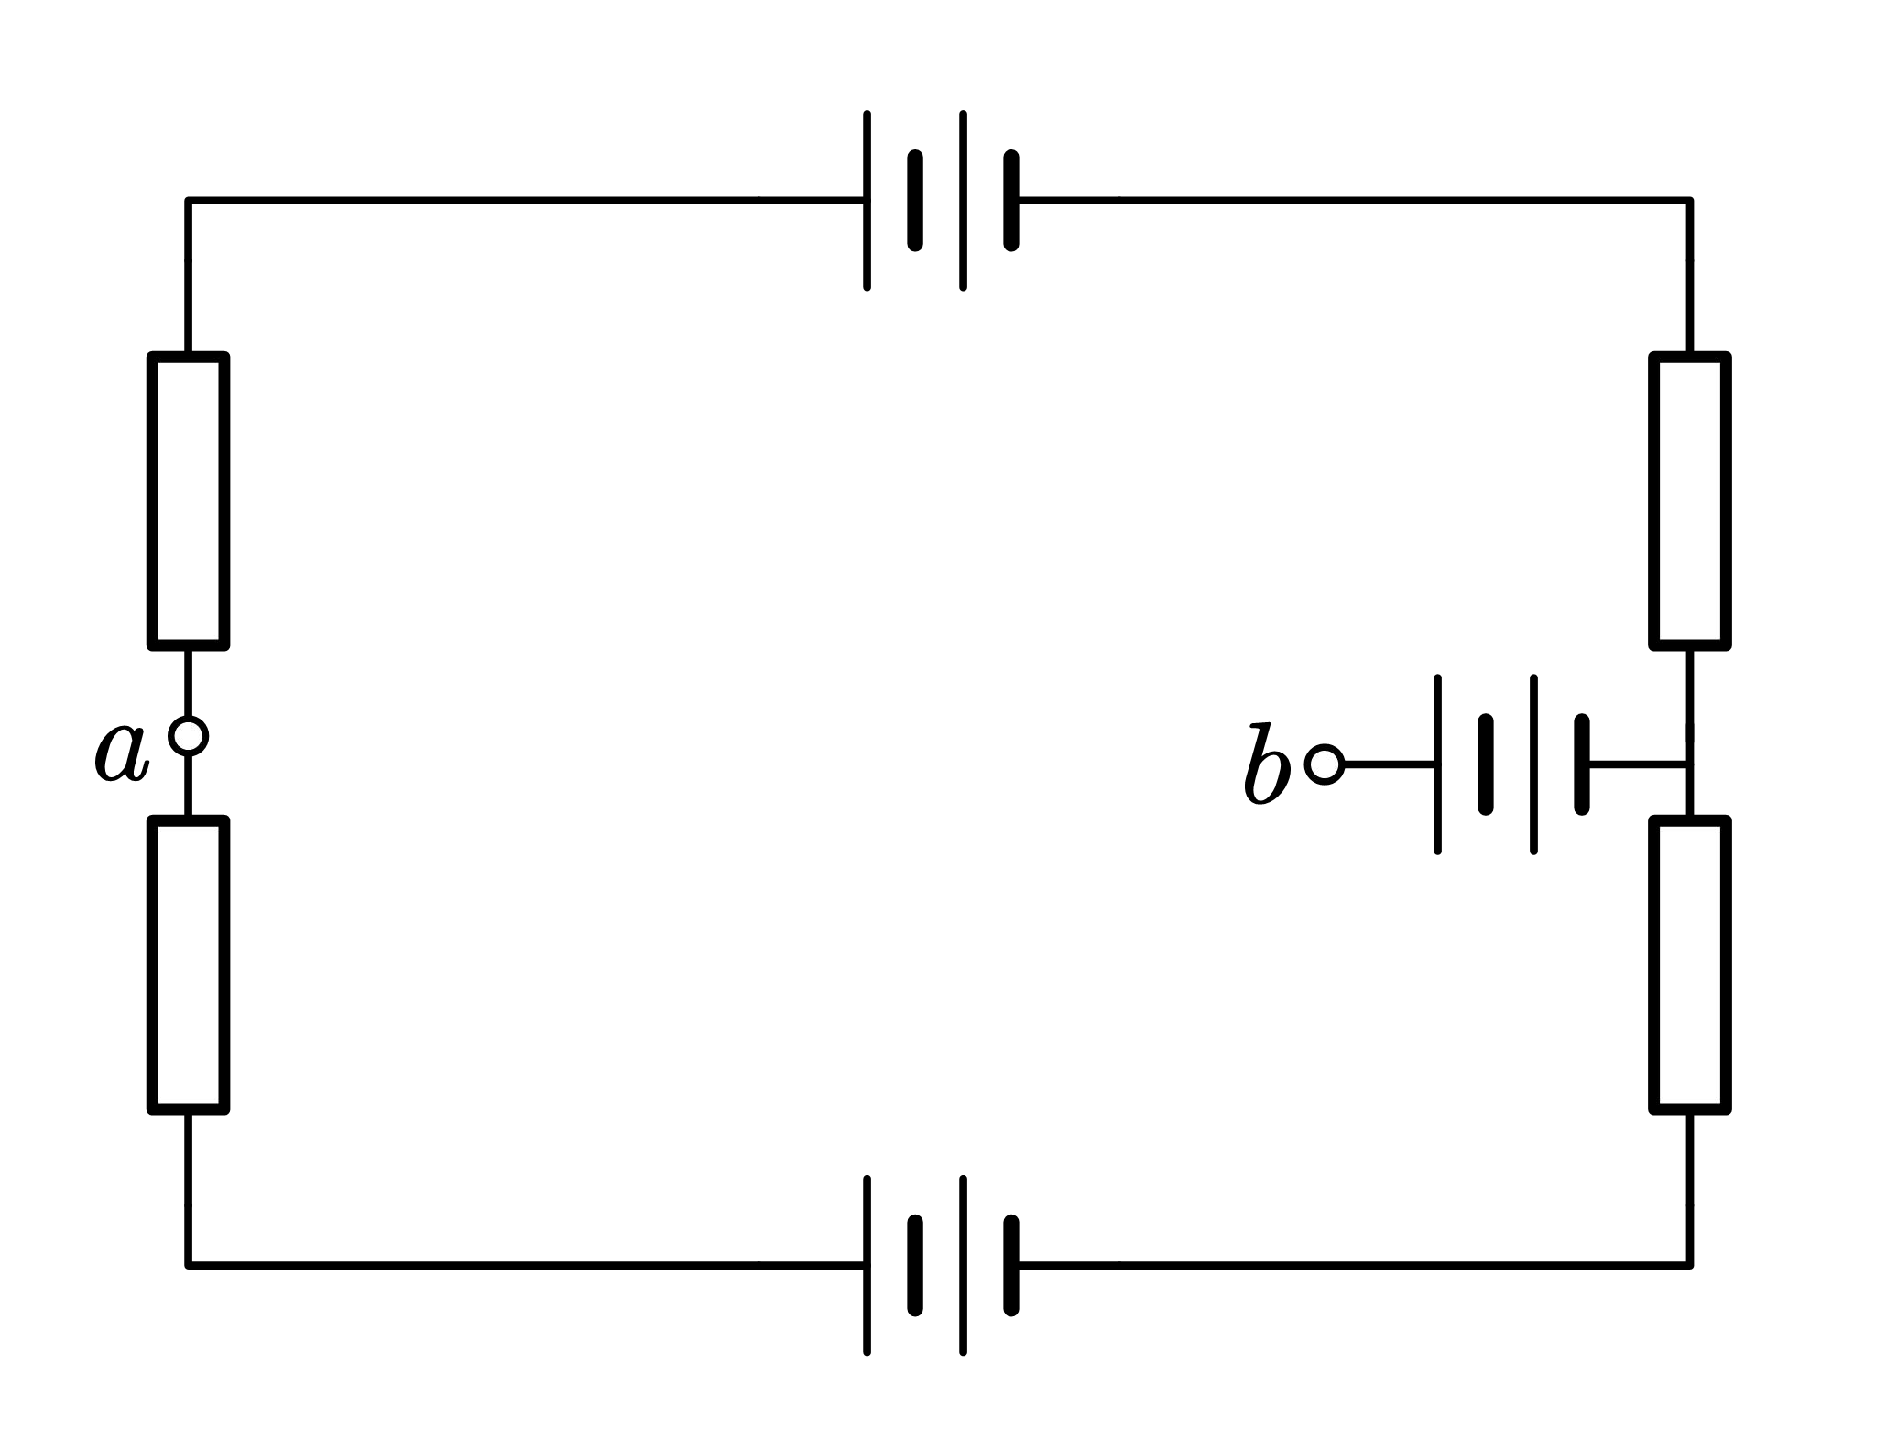
\includegraphics[width=0.3\linewidth]{../EarlyPic/3-21}
		\label{fig:3-21}
	\end{center}
	And as a result:
	$$
	U_{ab}=I(R_3+r_3+R_4)+\mathscr{E}_3-\mathscr{E}_2=\dfrac{\mathscr{E}_1-\mathscr{E}_2}{R_1+R_3+R_4+R_5+r_1+r_3}(R_3+r_3+R_4)+\mathscr{E}_3-\mathscr{E}_2=1\thinspace\mathrm{V}
	$$
	
	\subsubsection*{(2)}
	Based on the principle of independent superposition of currents:
	
	% TODO: \usepackage{graphicx} required
		\begin{center}
				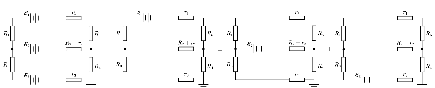
\includegraphics[width=1\linewidth]{../LatePic/3-21-(2)}
			\label{fig:3-21-2}
		\end{center}
	
	\begin{align*}
		I_1&=\frac{\mathscr{E} _1}{\left( R_2+r_2 \right) //\left( R_3+r_3+R_4 \right) +\left( R_1+r_1+R_5 \right)}\frac{R_3+r_3+R_4}{\left( R_3+r_3+R_4 \right) +\left( R_2+r_2 \right)}
		\\
		I_2&=-\frac{\mathscr{E} _2}{\left( R_2+r_2 \right) +\left( R_1+r_1+R_5 \right) //\left( R_3+r_3+R_4 \right)}
		\\
		I_3&=\frac{\mathscr{E} _3}{\left( R_3+r_3+R_4 \right) +\left( R_1+r_1+R_5 \right) //\left( R_2+r_2 \right)}\frac{R_1+r_1+R_5}{\left( R_1+r_1+R_5 \right) +\left( R_2+r_2 \right)}
		\\\\
		I&=I_1+I_2+I_3
		\\
		&=\frac{\mathscr{E} _1}{\left( R_2+r_2 \right) //\left( R_3+r_3+R_4 \right) +\left( R_1+r_1+R_5 \right)}\frac{R_3+r_3+R_4}{\left( R_3+r_3+R_4 \right) +\left( R_2+r_2 \right)}
		\\
		&\quad-\frac{\mathscr{E} _2}{\left( R_2+r_2 \right) +\left( R_1+r_1+R_5 \right) //\left( R_3+r_3+R_4 \right)}
		\\
		&\quad+\frac{\mathscr{E} _3}{\left( R_3+r_3+R_4 \right) +\left( R_1+r_1+R_5 \right) //\left( R_2+r_2 \right)}\frac{R_1+r_1+R_5}{\left( R_1+r_1+R_5 \right) +\left( R_2+r_2 \right)}
		\\
		&=\dfrac{2}{13}\thinspace\mathrm{A}
	\end{align*}
	\subsection*{3-26}
	Do as above we can have
	$$
	\mathscr{E}_1=18\thinspace\mathrm{V}\qquad\mathscr{E}_2=7\thinspace\mathrm{V}\qquad U{ab}=13\thinspace\mathrm{V}
	$$
	\subsection*{3-28}
	\subsubsection*{(1)}
	Consider using the full circuit Ohm's law after the capacitor is disconnected.
	$$
	I=\frac{10\thinspace\mathrm{V}+20\,\mathrm{V}-24\,\mathrm{V}}{2.0\,\Omega +10\,\Omega +3.0\,\Omega +17\,\Omega +18\,\Omega}=0.12\,\mathrm{A}
	$$
	So $U_A=-(18+2.0)\,\Omega\times0.12\,\mathrm{A}+10\,\mathrm{V}=7.6\,\mathrm{V}$.
	\subsubsection*{(2)}
	Consider the node is $U_x$.
	$$
	\left( U_x-U_A \right) \times 20\,\upmu\mathrm{F}+\left( U_x-U_B \right) \times 20\,\upmu\mathrm{F}+U_x\times 10\,\upmu\mathrm{F}=0
	$$
	As a result.
	$$
	Q=U_x\times10\,\upmu\mathrm{F}=136\,\upmu\mathrm{C}
	$$
	That means the $U_x>0$, so the plane is $-136\,\upmu\mathrm{C}$.
\end{document}

